\documentclass[master.tex]{subfiles}
\begin{document}

\chapter{Example Formal System - Typed Lambda Calculus}
\label{chap:example_lambda_calculus}

Chapters \ref{chap:example_simple_arithmetic} and
\ref{chap:example_propositional_logic} show most of features and usability of
\emph{Phometa} already so this chapter aims to show that Phometa is powerful
enough as it can even encode more complex formal system like \emph{typed lambda
  calculus}. Hence, it is clear that Phometa is suitable to encode most of
formal system that user can think of.

Credit: Some of material here modified from lecture note of ``382 --- Type
Systems for Programming Languages'' (third year course), Department of
Computing, Imperial College London. Thank you Dr Steffen van Bakel for this.

Please note that the following formal system is just a faction of what Lambda
Calculus could be. To be precise, this formal system includes $\beta$-reduction
and simply types of Lambda Calculus.

\section{Terms and Variables}

Lambda Calculus stimulates computational model in functional manner. Basically,
it will have a grammar \pgmr{Term} which can be either a
\pgmr{Variable}, an anonymous function, an application, or a substitution.
It can be described in Backus-Naur Form like this


\begin{center}
    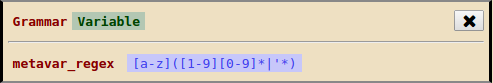
\includegraphics[width=0.7\textwidth]{lamb-gmr-var}
\end{center}

\begin{figure}[H]
    \centering

\begin{minipage}{0.7\textwidth}
    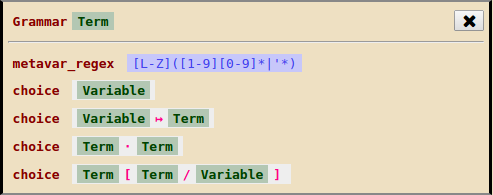
\includegraphics[width=\textwidth]{lamb-gmr-term}
\end{minipage}

\caption{Definition of \pgmr{Variable} and \pgmr{Term}}
\end{figure}

The first choice of \pgmr{Term} represents variable which you can think as a
mark point that other terms can refer to.

The second choice of \pgmr{Term} represents an anonymous function i.e.\
\term{lamb-etc-1} means a function that get a variable \pvar{x} and return a
term \pvar{M} where \pvar{M} might contain \pvar{x}. From now on, I will call as
``blinder''

An anonymous function is usually represented by \term{lamb-etc-2} but I use
\term{lamb-etc-1} since it works better with underlines when we implement it in
Phometa.

The third choice of \pgmr{Term} represents an application i.e. \term{lamb-etc-3}
means apply term \pvar{M} to term \pvar{N} where \pvar{M} usually be an
anonymous function\footnote{Or will become anonymous function after evaluate the
  term.}.

The fourth choice of \pgmr{Term} represents a substitution i.e.\
\term{lamb-etc-4} means a term \pvar{M} that every occurrence of free variable
\pvar{x} will be replaced by a term \pvar{N}.

A variable \pvar{x} is free variable if it doesn't live inside an anonymous function
that has \pvar{x} as blinder\footnote{Blinder is a variable on the left hand side
of $\mapsto$ of an anonymous function}, otherwise, it is bounded variable.



\section{Side Conditions}
Sometime we want to build a simple formal system but its dependency relies on
more complex formal system, for example, $\beta$ reduction (will be defined
later) needs to check whether a variable is a free variable of a curtain term or
not, and checking free variable require knowledge of sets. Normally we should
build a formal system regarding to set, then we can build $\beta$ reduction,
however this is overkill as formal system of set is much larger than $\beta$
reduction. To solve this problem, we can build a grammar that construct a
statement that need to be judge by the user as the following

\begin{figure}[H]
    \centering
\begin{minipage}{0.7\textwidth}
    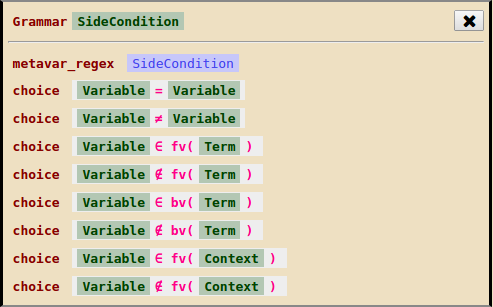
\includegraphics[width=\textwidth]{lamb-gmr-sidecond}
\end{minipage}
\caption{Definition of \pgmr{SideCondition}}
\end{figure}

Then write a single rule that allow to prove any side condition.

\begin{figure}[H]
    \centering
\begin{minipage}{0.7\textwidth}
    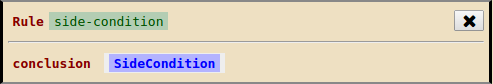
\includegraphics[width=\textwidth]{lamb-rule-sidecond}
\end{minipage}
\caption{Definition of \prule{side-condition}}
\end{figure}

Every time when \pgmr{SideCondition} appear in a derivation tree, user needs
extra care and determine whether that side condition holds or not. If it holds
then apply \prule{side-condition} and it is done. Please note that there is no
mechanism to prevent user to apply \prule{side-condition} on a false
\pgmr{SideCondition} and it will result in inconsistency, in another word, by
using side condition technique, we \emph{trust} user to do the right thing.

\section{$\beta$ Reduction}

Since \pgmr{Term} represents computational model, so it can be
\emph{evaluated}. A step of evaluation in Lambda Calculus is called
\pgmr{$\beta$-Reduction} which can be defined as the following

\begin{figure}[H]
    \centering
\begin{minipage}{0.7\textwidth}
    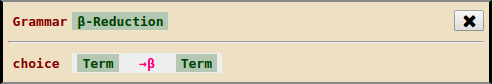
\includegraphics[width=\textwidth]{lamb-gmr-beta}
\end{minipage}
\caption{Definition of \pgmr{$\beta$-Reduction}}
\end{figure}

\term{lamb-etc-5} means \pvar{M} can reduce to \pvar{N} in one step, the
rules to control this can be defined as the following

\begin{figure}[H]
    \centering

\begin{minipage}{0.48\textwidth}
\begin{flushleft}
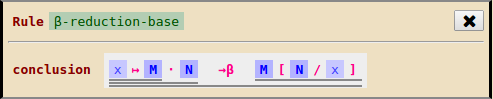
\includegraphics[width=\textwidth]{lamb-rule-beta-1}
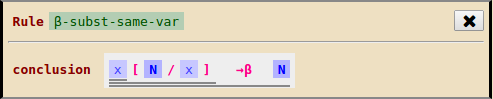
\includegraphics[width=\textwidth]{lamb-rule-beta-2}
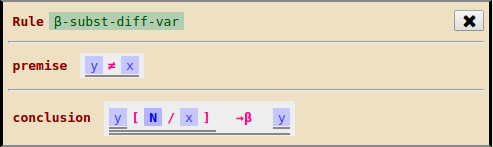
\includegraphics[width=\textwidth]{lamb-rule-beta-3}
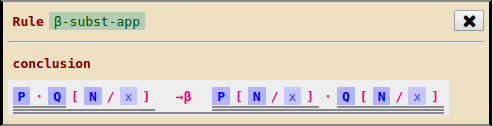
\includegraphics[width=\textwidth]{lamb-rule-beta-4}
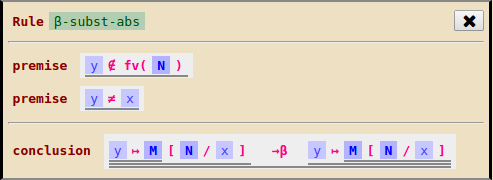
\includegraphics[width=\textwidth]{lamb-rule-beta-5}
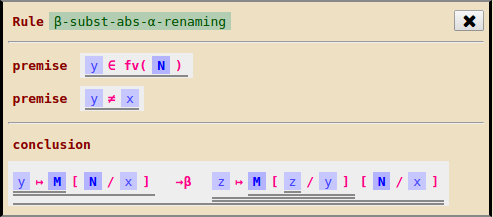
\includegraphics[width=\textwidth]{lamb-rule-beta-6}
\end{flushleft}
\end{minipage}
~
\begin{minipage}{0.48\textwidth}
\begin{flushright}
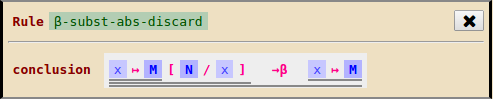
\includegraphics[width=\textwidth]{lamb-rule-beta-7}
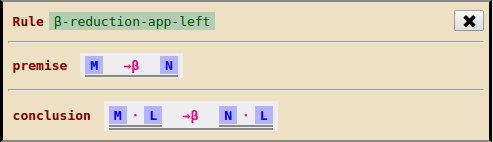
\includegraphics[width=\textwidth]{lamb-rule-beta-8}
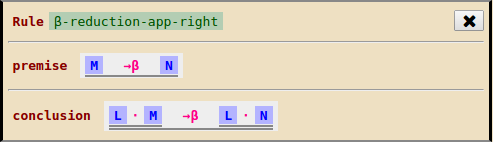
\includegraphics[width=\textwidth]{lamb-rule-beta-9}
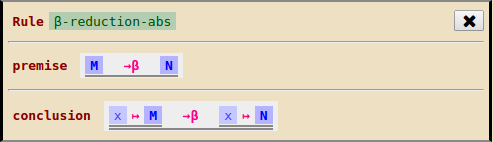
\includegraphics[width=\textwidth]{lamb-rule-beta-10}
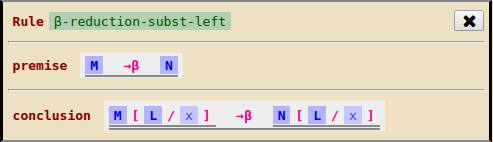
\includegraphics[width=\textwidth]{lamb-rule-beta-11}
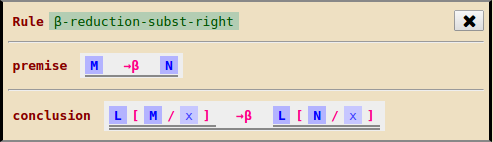
\includegraphics[width=\textwidth]{lamb-rule-beta-12}
\end{flushright}
\end{minipage}

    \caption{Rules for \pgmr{$\beta$-Reduction}}
\end{figure}

\newpage

There is also \texttt{$\beta$-ManyReduction} which reflexive transitive closure
of \texttt{$\beta$-Reduction}.

\begin{figure}[H]
    \centering
\begin{minipage}{0.48\textwidth}
\begin{flushleft}
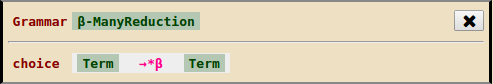
\includegraphics[width=\textwidth]{lamb-gmr-betamany}
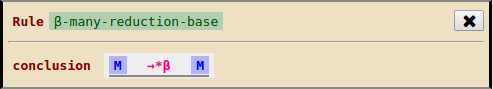
\includegraphics[width=\textwidth]{lamb-rule-betamany-1}
\end{flushleft}
\end{minipage}
~
\begin{minipage}{0.48\textwidth}
\begin{flushright}
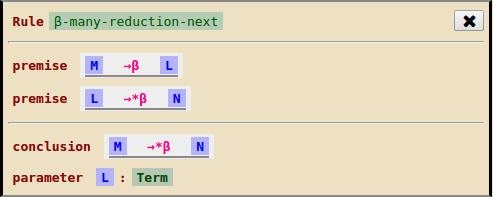
\includegraphics[width=\textwidth]{lamb-rule-betamany-2}
\end{flushright}
\end{minipage}

\caption{Definition of \pgmr{$\beta$-ManyReduction} and its rules}
\end{figure}

Now we are ready to build a derivation tree,

\begin{figure}[H]
    \centering
\begin{minipage}{\textwidth}
    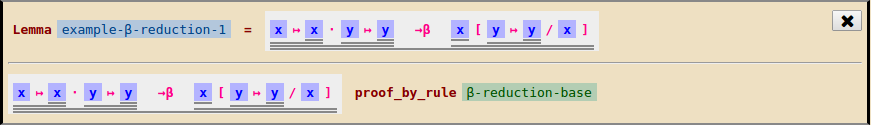
\includegraphics[width=\textwidth]{lamb-red-1}
    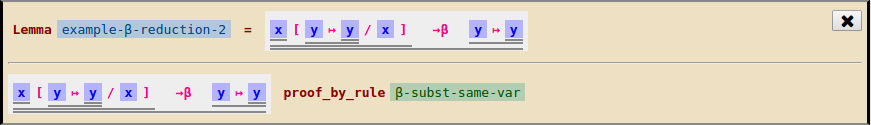
\includegraphics[width=\textwidth]{lamb-red-2}
    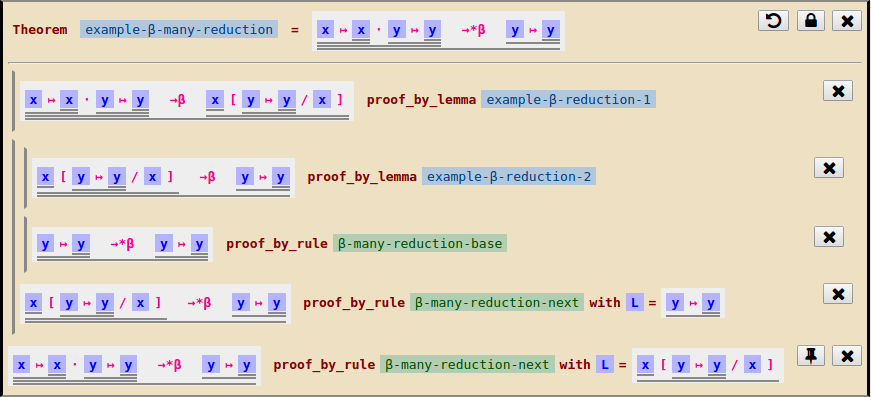
\includegraphics[width=\textwidth]{lamb-red-3}
\end{minipage}
\caption{Examples of derivation trees of \pgmr{$\beta$-Reduction} and \pgmr{$\beta$-ManyReduction}}
\end{figure}

\section{Simply Types}

Some terms can be reduced infinitely many times e.g.
\term{lamb-loop-1} \term{lamb-loop-0} \\
\term{lamb-loop-2} \term{lamb-loop-0}
\term{lamb-loop-3} \term{lamb-loop-0} \\
\term{lamb-loop-4} \term{lamb-loop-0}
\term{lamb-loop-1} \term{lamb-loop-0} $\cdots$

This is not desirable as it implies a program that will never terminate. To
solve this problem we can try to find a type of a term, if found, we know that
the term as finite number of reductions. \pgmr{Type} can be defined as the
following

\begin{figure}[H]
    \centering
\begin{minipage}{0.7\textwidth}
    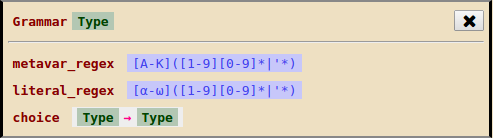
\includegraphics[width=\textwidth]{lamb-gmr-type}
\end{minipage}
\caption{Definition of \pgmr{Type}}
\end{figure}

\vspace{-2em}
\pgmr{Type} can be instantiated as
\begin{itemize}
\item meta variable --- for generic type which can be used in another place.
\item literal --- for constant type similarly to Int, Bool, Char, etc.
\item \term{lamb-etc-7} --- a type of anonymous function that receive input
  of type \pvar{A} and return output of type \pvar{B}.
\end{itemize}

To state that a term has the particular type we can use \pgmr{Statement},
and in order to prove a that \pgmr{Statement} holds under certain
assumptions, we need \pgmr{Context} and \pgmr{Judgement}. These three
grammars can be defined as the following

\begin{figure}[H]
    \centering
\begin{minipage}{0.6\textwidth}
    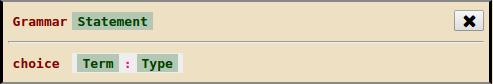
\includegraphics[width=\textwidth]{lamb-gmr-statement}
    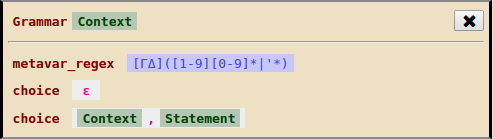
\includegraphics[width=\textwidth]{lamb-gmr-context}
    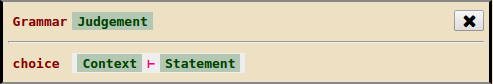
\includegraphics[width=\textwidth]{lamb-gmr-judgement}
\end{minipage}
\caption{Definition of grammars related to \pgmr{Type}}
\end{figure}

The rules regarding to type can be defined as the following,
\vspace{-1em}
\begin{figure}[H]
    \centering
\begin{minipage}{0.5\textwidth}
    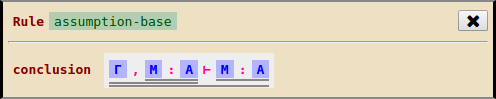
\includegraphics[width=\textwidth]{lamb-rule-type-1}
    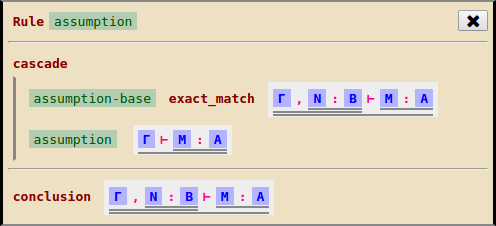
\includegraphics[width=\textwidth]{lamb-rule-type-2}
    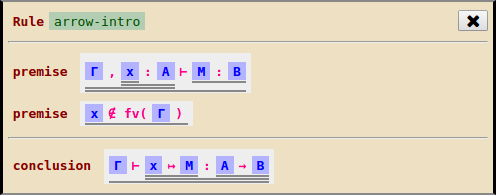
\includegraphics[width=\textwidth]{lamb-rule-type-3}
    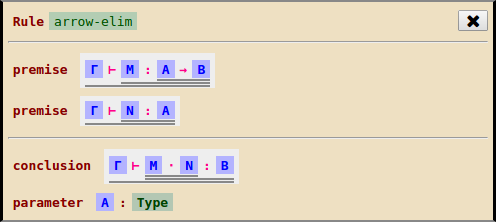
\includegraphics[width=\textwidth]{lamb-rule-type-4}
    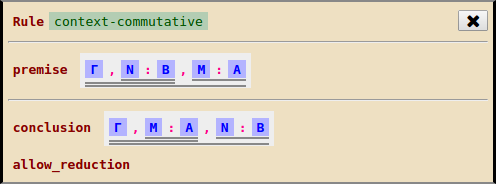
\includegraphics[width=\textwidth]{lamb-rule-type-5}
    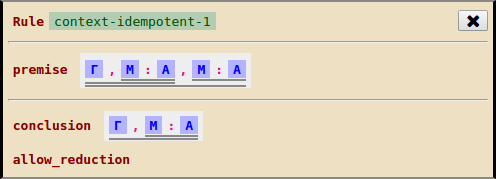
\includegraphics[width=\textwidth]{lamb-rule-type-6}
    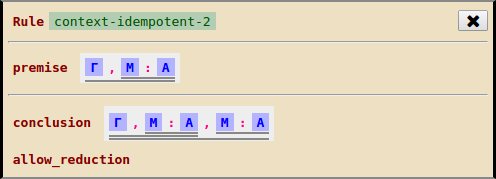
\includegraphics[width=\textwidth]{lamb-rule-type-7}
\end{minipage}
\caption{Definition of rules using for type resolution.}
\end{figure}

Now we are ready to build a derivation tree,

\begin{figure}[H]
    \centering
\begin{minipage}{\textwidth}
    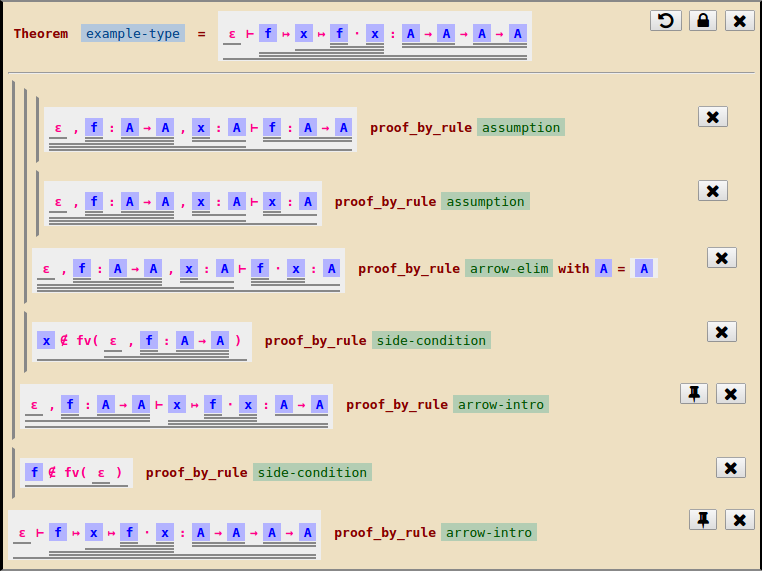
\includegraphics[width=\textwidth]{lamb-thm-type}
\end{minipage}
\caption{Examples of derivation trees of \pgmr{Judgement}.}
\end{figure}

\end{document}